\documentclass[12pt,letterpaper]{article}
\usepackage[utf8]{inputenc} %Codificacion del texto (ISO Latin1 encoding)
\usepackage{graphicx} %Permite exportar imagenes en formato eps
\usepackage{fancyhdr} %Permite acomodar a tu gusto la parte de arriba y
\usepackage[hmargin=1in,vmargin=1in, lmargin=1in, rmargin=1in]{geometry}
\usepackage[final]{pdfpages}
\usepackage{amssymb}
\usepackage{amsmath}


\pagestyle{fancyplain}

\lhead{\it Segundo Semestre del 2009} %Parte superior izquierda
\rhead{\bf \it Propuesta de Proyecto} %Parte superior derecha
\lfoot{} %Parte inferior izquierda. \thepage indica
% el numero de pagina
\cfoot{} %Parte inferior central
\rfoot{\bf \thepage} %Parte inferior derecha
\renewcommand{\footrulewidth}{0.4pt} %Linea de separacion inferior

\title{Propuesta de Proyecto}

\author{Esteban Bombal, Rodrigo Fernández, Cristián Maureira,\\Ignacio Villacura y Gabriel Zamora}
\begin{document}
\bibliographystyle{plain}
\maketitle\thispagestyle{empty}

\section{Antecedentes}
\label{op:antecedentes}
\begin{itemize}
	\item \textbf{Título del proyecto:} Autenticación JAAS para máquinas JBoss

	\item \textbf{Equipo de trabajo:}\\
	\begin{center}
	%(Nombre y RUT de cada integrante; identifique al jefe de proyecto y lístelo en primer lugar)
		\renewcommand{\arraystretch}{2}
		\begin{tabular}{|c|c|}
		\hline
		\textbf{Nombre} & \textbf{Rut}\\
		\hline
		Esteban Bombal $\dagger$& 16.557.976-3\\
		\hline
		Ignacio Villacura & 16.792.342-9\\
		\hline
		Cristián Maureria & 16.759.352-6\\
		\hline
		Gabriel Zamora	& 16.331.227-1\\
		\hline
		Rodrigo Fernández  &  16.812.081-8\\
		\hline
		\end{tabular}
		\\
		\vspace{0.5cm}
	\small $\dagger$ Jefe de Proyecto
	\end{center}
\end{itemize}

\newpage

\section{Resumen}
\label{target:resumen}
%Escriba un resumen en un máximo de 30 líneas. Debe ser lo suficientemente informativo,
%presentado el trabajo que pretenden desarrollar, conteniendo una descripción de los principales
%puntos que se abordarán, objetivos, metodología y resultados esperados.
El presente informe aborda lo que será el proyecto de \textbf{Control de Acceso Lógico} para el servidor de aplicaciones \textbf{JBoss}.
Nuestro grupo de trabajo enfocará el proyecto de \textbf{Taller de Sistemas de Computación} en la implementación de un framework
de seguridad basado en Java, llamado \textbf{JAAS}. Gracias a esta herramienta, el grupo logrará entablar una conexión a servicios de directorios mediante \textbf{LDAP} para la conexión a la máquina \textbf{JBoss} correspondiente.

Se plantean en este informe metodologías de trabajo estructuradas para el correcto término de este proyecto.
Existirán horarios semanales de trabajo dispuesto exclusivamente en el avance del proyecto, así como reuniones
semanales donde se revisará el avance de cada área de trabajo, así como las dudas surgentes y nuevas tareas que puedan
aparecer. Además el grupo contará con medios establecidos de comunicación, como lo son el uso de \textbf{Trac} para estados de avance,
\textbf{Alias de Correo} para comunicados generales, y el software \textbf{Skype} para comunicación inmediata con los integrantes del grupo.


\newpage

\section{Formulación general del proyecto}
\label{team:formulacion}
%En un máximo de 3 páginas formule en forma general su proyecto, donde usted se debe referir a
%los siguientes puntos:

\subsection{Definición del Problema}
	%Defina el contexto y el problema que pretende abordar en el marco de este proyecto. Incluya una
	%discusión bibliográfica que fundamente adecuadamente desde el punto de vista técnico su
	%proyecto.
	Siempre que existe una relación de cualquier tipo entre dos o más entidades,
	está la posibilidad que el \emph{medio} utilizado para la comunicación,
	sea perturbado por cualquier actividad fuera de dicho universo de conversación,
	como lo muestra la figura ~\ref{fig:fig1}.

	\begin{figure}[htp]
		\centering
		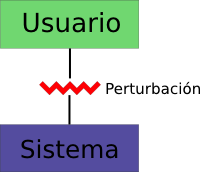
\includegraphics[scale=0.3]{img/user-sist}
		\caption{Comunicación Usuario-Sistema y sus perturbaciones}
		\label{fig:fig1}
	\end{figure}

	En el área de la informática, el manejo de información es un tema latente
	en todo sentido, por lo tanto para poder mantener la credibilidad y veracidad de
	dicha información, es necesario poder asegurar el medio de intercambio de datos,
	es aquí donde aparece el término de \emph{Control de Acceso Lógico},
	enfocado a sistemas y aplicaciones, siendo así la primera barrera a cualquier
	\emph{perturbación} que nuestro ambiente de transferencia de información pueda
	ser afectado.

	Para poder reducir la probabilidad de que las \emph{perturbaciones} tengan éxito,
	y puedan interferir la transferencia de información, se utilizan distintos métodos
	seguridad, ya sea mediante hardware, software o ambos, todos con el mismo fin de
	impedir un acceso inseguro.

	Es por lo dicho anteriormente que los \emph{Controles de Acceso lógico} son de vital
	importancia, pues permiten proteger los recursos en una amplia variedad de sistemas.
	Debido a la problemática señalada anteriormente, han llegado a surgir distintos tipos
	de sistemas para poder hacer interactuar herramientas y así establecer un cierto control
	en nuestro canal de comunicación, como es el caso del servicio del \emph{Java
	Authentication and Authorization Service}~\cite{paper1} que nos permite tener acceso a
	servicios de control de autenticación y acceso para distintas aplicaciones Java,
	sin dejar de lado algunos otros tipos de utilización,
	como lo es el caso de poder ayudar a remover ambigüedades de ciertas definiciones informales
	en un modelo de control, basado en una aplicación Java, convirtiéndola en una especie
	de máquina abstracta que se comporta bajo un conjunto de reglas~\cite{paper2}.

	Finalmente, cabe señalar que nuestra problemática aumenta notablemente cuando los recursos de
	nuestro sistema almacenan datos extremadamente sensibles, como ``información confidencial'',
	``documentos clasificados'', etc, por ésto es que claramente para solucionar nuestra situación
	necesitamos un sistema robusto, estableciendo alguna suerte de credenciales virtuales,
	para realizar ciertas autenticaciones, conteniendo así la información necesaria para poder
	autenticar a un sujeto frente a un servicio determinado~\cite{paper3}.
	

\subsection{Objetivos del Proyecto}
	%Defina el objetivo general del proyecto y los objetivos específicos que han identificado (detalle de
	%lo que quieren alcanzar), limitando adecuadamente el alcance del proyecto (qué cosas
	%definitivamente no abordarán).
	El objetivo principal de nuestro proyecto es:

\begin{itemize}
\item Implementar el modelo API de autenticación JAAS (Java Authentication and Authorization Service) para controlar el acceso, vía autenticación, a máquinas JBoss, a cargo del grupo 5. 
\end{itemize}
	Nuestros objetivos específicos son:

\begin{itemize}
\item Poder comunicarse con un Servidor de Directorios, como LDAP, o utilizar una base de datos para almacenar la información de los usuarios.
\item Utilizar JAAS, para autentificar vía  web a los usuarios que quieran ingresar a la máquina JBoss.
\item Dar acceso diferenciado a los usuarios, ya sean administrador o usuarios, para poder utilizar la maquina JBoss.
\end{itemize}

	Si bien abordaremos las bases de la autenticación, hay algunos puntos los cuales, por disponibilidad de tiempo, no podemos comprometernos a realizar, correspondiendo a las herramientas mas avanzadas de JAAS como:

\begin{itemize}
\item Autenticaciones múltiples bajo un solo dominio.
\item No utilizaremos JPam para la autenticación.
\end{itemize}

	
\subsection{Resultados Esperados}
	%Refiérase brevemente a los resultados que espera lograr con este trabajo y relaciónelos con los
	%entregables que debe contener el informe final; especialmente con el reporte técnico, material
	%complementario y demostración.
	Para nuestro proyecto pretendemos lograr implementar un sistema de autenticación JAAS, de manera
óptima para poder realizar las tareas de comunicación con un Sistema de Directorios, como LDAP, y
permitir la autenticación diferenciada en el ingreso a la máquina JBoss que implementarán nuestros
compañeros del grupo correspondiente. Esperamos comprender el sistema a fondo, utilizando las correctas
directrices de seguridad que éste posee y dar un servicio óptimo de autenticación de usuarios para los
demás grupos que utilicen el sistema.
	
También, y a pesar de no estar en nuestros objetivos específicos, podríamos probar la implementación de
JAAS en otros servicios de autenticación como Pam, a través del puente que proporciona JPam y comparar
las ventajas y desventajas que estos dos sistemas poseen y ver como a su vez se puedan ver
complementados.
		



\newpage

\section{Planificación del Proyecto}
\label{prod:planificacion}
%En un máximo de 2 páginas formule la planificación de su proyecto, donde usted se debe referir a
%los siguientes puntos.

\subsection{Metodología de Trabajo}
	%Señale los enfoques y procedimientos a ser usados en el desarrollo del proyecto. Especifique cómo
	%piensa trabajar para lograr todos los objetivos propuestos. Refiérase a cómo se organizará el
	%equipo de trabajo, responsabilidades asumidas por cada miembro, y qué medios de comunicación
	%y de toma de decisiones emplearán.


Nuestro equipo ha trabajado anteriormente en muchas otras actividades, tanto académicas como con otros
proyectos, por lo que para el desarrollo del proyecto pensamos continuar usando la siguiente metodología
de trabajo:
\begin{description}
	\item[\textbf{Horarios Semanales de trabajo:}] 
		Se coordinarán horarios de trabajo en grupo para asegurar tiempo de trabajo en el proyecto
		durante la semana.

	\item[\textbf{Reuniones presenciales:}]
		Cada semana nos reuniremos en un horario definido a revisar los avances de cada uno y resolver
		los problemas que vayan ocurriendo.

	\item[\textbf{Coordinación y asignación de metas semanales:}]
		Cada semana se asignarán las metas y tareas a cumplir cada semana, las cuales serán evaluadas
		durante las reuniones presenciales.

	\item[\textbf{Worklogs:}]
		Se deberá dejar un registro de toda actividad realizada, indicando el día y
		el detalle de lo realizado en el Trac habilitado para el proyecto.

\end{description}



\subsection{Plan de Trabajo}
	%Coherentemente con la definición de sus objetivos y la metodología de trabajo, identifique las
	%tareas que desarrollará en el contexto del proyecto. Refiérase a la distribución y asignación de
	%tareas entre los miembros del equipo. Construya una carta Gantt con las principales tareas y los
	%hitos que debe cumplir en el desarrollo del proyecto.
En el presente plan de trabajo, se enlistan las actividades a realizar en este proyecto y sus participantes:
\small
\begin{itemize}
\item Investigación \emph{(Todos)}
\begin{itemize}
	\item JBOSS
	\item Documentación Básica
	\item Uso y aplicación de JAAS en JBOSS
	\item JAAS 
	\item Documentación Básica
	\item Distintos tipos de Uso
	\item Funcionamiento Cliente-Servidor
	\item Sign-On
	\item Políticas de Seguridad
	\item LDAP
	\item Integración LDAP con JAAS
\end{itemize}
\item Implementación
\begin{itemize}
	\item Implementación simple de plataforma JBOSS \emph{(Rodrigo Fernández y Cristian Maureira)}
	\item Implementación simple de protocolo LDAP \emph{(Gabriel Zamora y Cristian Maureira)}
	\item Implementación de Single Sign-On en JAAS \emph{(Rodrigo Fernández y Ignacio Villacura)}
	\item Implementación de servicio JAAS \emph{(Ignacio Villacura y Esteban Bombal)}
	\item Desarrollo y uso de JAAS en JBOSS usando LDAP \emph{(Gabriel Zamora y Esteban Bombal)} 
	\item Desarrolo servicio web sobre JBOSS \emph{(Rodrigo Fernandez e Ignacio Villacura)}
	\item Integración de JAAS y LDAP \emph{(Cristian Maureira y Esteban Bombal)}
	\item Integración de servicio web y JAAS \emph{(Gabriel Zamora y Esteban Bombal)}
	\item Testing y Debugging \emph{(Rodrigo Fernandez)}
\end{itemize} 
\item Integración entre proyectos 
\begin{itemize}
	\item Integración con proyecto LDAP \emph{(Cristian Maureira y Esteban Bombal)}
	\item Integración con proyecto JBOSS \emph{(Gabriel Zamora e Ignacio Villacura)}
\end{itemize}
\item Entregables \emph{(Rodrigo Fernández)}
\begin{itemize}
	\item Primer Informe de Avance (5-10-09) 
	\item Segundo Informe de Avance (2-11-09) 
	\item Informe de Gestión del Proyecto 
	\item Reporte Técnico
\end{itemize} 
\item Otros 
\begin{itemize}
	\item Mantención Bitácora 
	\item Mantención Carta Gantt 
\end{itemize}
\end{itemize}


Para mas detalle, ver la Carta Gantt en el anexo.\\


\subsection{Recursos}
	%Para el desarrollo de cualquier proyecto es necesario disponer de recursos tales como
	%documentación bibliográfica, software, hardware, y otros. En el caso particular de su proyecto,
	%especifique los recursos necesarios que ustedes requieren para desarrollarlo. Identifique los
	%recursos que ya tienen disponibles y cuáles deben adquirir.

A continuación, se identifican los principales recursos técnicos a utilizarse durante el desarrollo.

Para la coordinación y comunicación del equipo, se utilizarán las siguientes herramientas:

\begin{itemize}
    \item Alias de Correo, Trac y Skype
\end{itemize}

El proyecto se desarrollará completamente sobre la plataforma Linux,
específicamente las plataformas Fedora y CentOS que son utilizada en los laboratorios en el cual el
equipo trabaja, el laboratorio de Sistemas Distribuidos y el laboratorio de Integración Tecnológica.

Los lenguajes de programación y asociados que serán utilizados son los siguientes:

\begin{itemize}
    \item  Java Platform, Enterprise Edition (JEE).
\end{itemize}

Las herramientas que se usarán para el desarrollo son en su totalidad aplicaciones OpenSource.
Se destacan las siguientes:

\begin{itemize}
    \item LDAP, Git, LaTeX, Vi IMproved (VIM) y Planner
\end{itemize}

Por último, el hardware a utilizar será 1 servidor del LabIT o LabSD para poder llevar a cabo las pruebas
del proyecto.


\newpage

\section{Anexo: Carta Gantt}
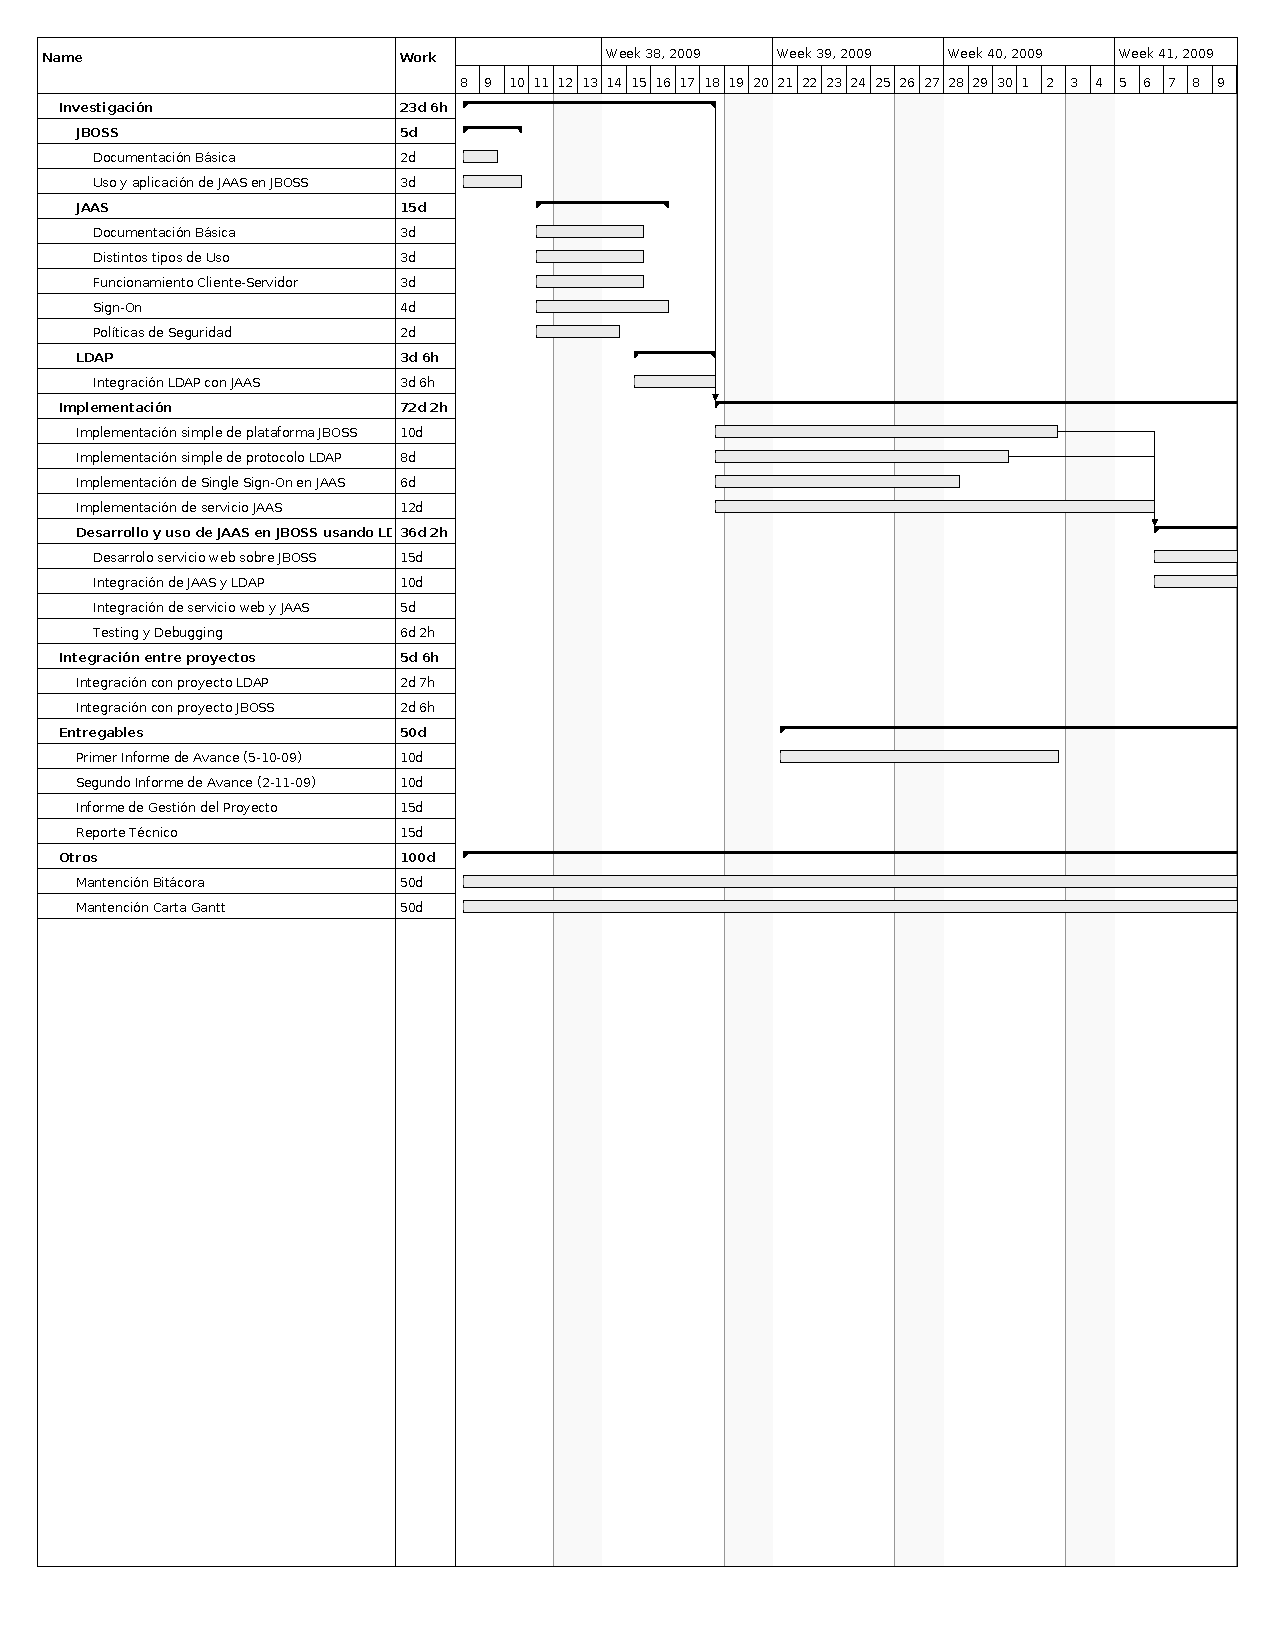
\includepdf[pages=-]{gantt.pdf}

\bibliography{propuesta}
\vfill \hfill CM/GZ/IV/EB/RF/DI/UTFSM/2009
\end{document}
